\documentclass{standalone}
\usepackage{tikz}
\usetikzlibrary{plotmarks}

\begin{document}

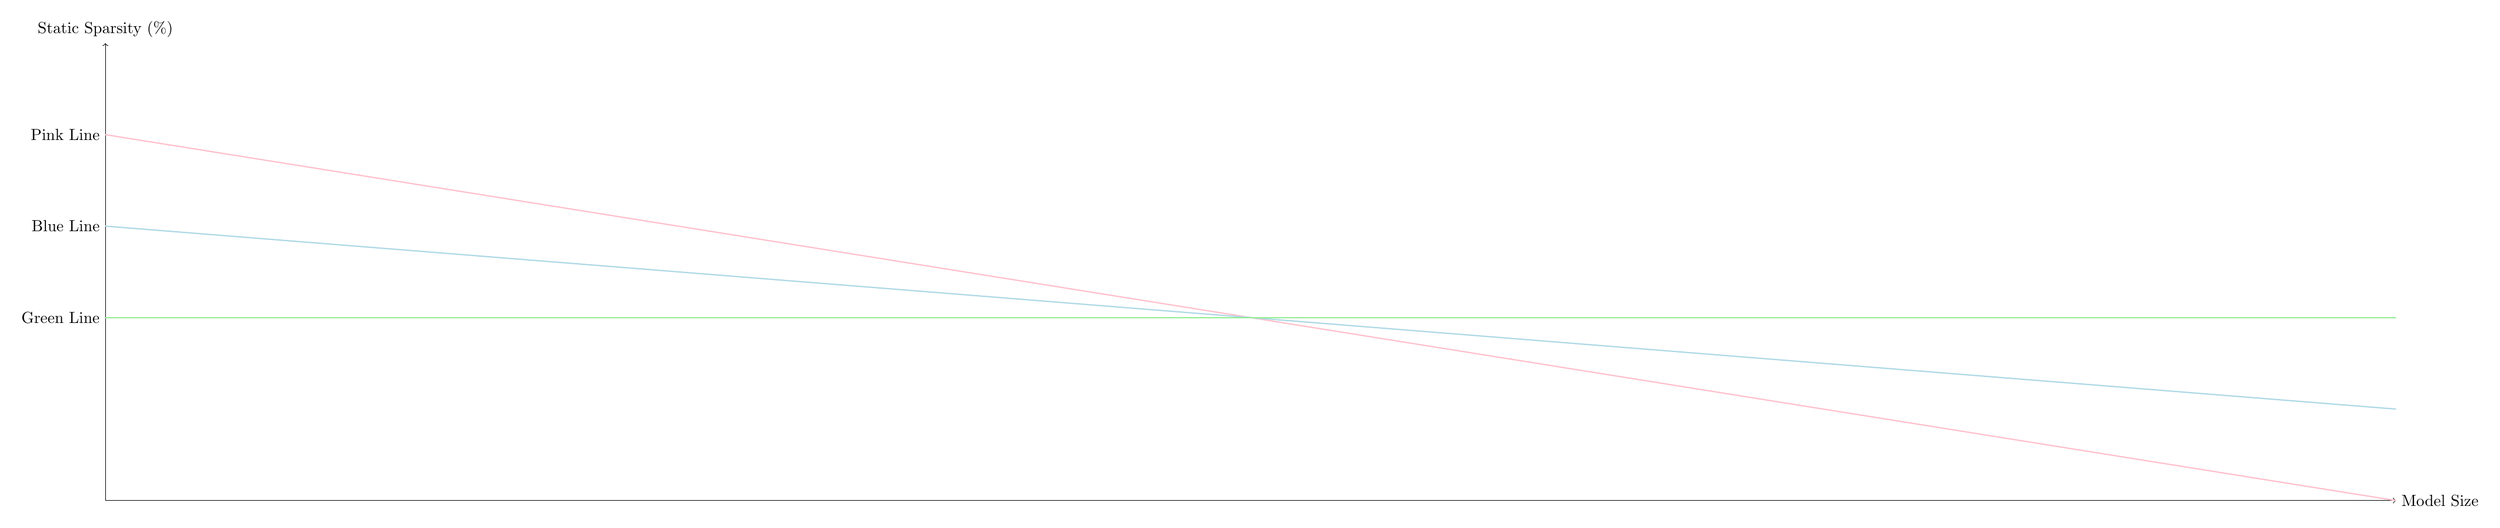
\begin{tikzpicture}[scale=1]
    % Define colors
    \definecolor{pink}{RGB}{255, 192, 203}
    \definecolor{blue}{RGB}{173, 216, 230}
    \definecolor{green}{RGB}{144, 238, 144}

    % Set up the axes
    \draw[->] (0,0) -- (50,0) node[right] {Model Size};
    \draw[->] (0,0) -- (0,10) node[above] {Static Sparsity (\%)};

    % Draw the lines
    \draw[color=pink, thick] plot coordinates {(0,8) (50,0)};
    \draw[color=blue, thick] plot coordinates {(0,6) (50,2)};
    \draw[color=green, thick] plot coordinates {(0,4) (50,4)};

    % Add labels
    \node at (0,8) [left] {Pink Line};
    \node at (0,6) [left] {Blue Line};
    \node at (0,4) [left] {Green Line};

    % Add legend
    \legend{Pink Line, Blue Line, Green Line}
\end{tikzpicture}

\end{document}